\subsection{Resonant Converters}
Resonant converters are a type of power converter that uses a resonant circuit to store energy and provide a smooth output voltage. These converters utilize resonant circuits, consisting of inductors, capacitors, and switches, to regulate the flow of energy. They are often used in applications where a high-quality, ripple-free output voltage is required.\\
The resonant frequency of the converter is determined by the values of the inductor and capacitor in the resonant circuit. The output voltage of the converter is also determined by the resonant frequency.\\
Resonant converters are more efficient than non-resonant converters, and they can produce a higher-quality output voltage. However, they are also more complex to design and build.

\subsection{Types of Converters and Why LLC}
Now there are various types of configurations of resonant converters possible.

\noindent
An ideal transformer has its magnetizing inductor in parallel with its input winding. This parallel magnetizing inductor can be used as part of the resonant circuit.
\begin{figure}[ht]
    \centering
    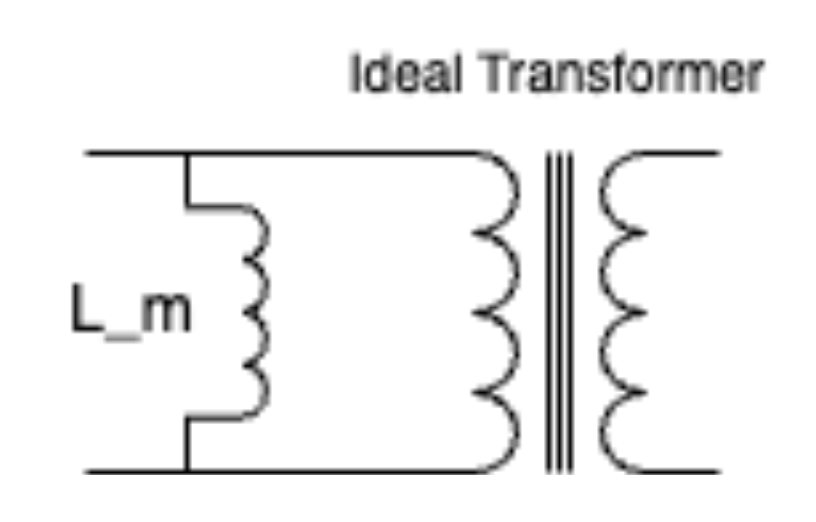
\includegraphics[width=0.3\textwidth]{basic1.png}
    \label{fig:basic1}
\end{figure}

\noindent
In the real world, a transformer always comes with a leakage inductor in series with the transformer windings. This series leakage inductor can also be used as a part of the resonant circuit that we intend to design.
\begin{figure}[ht]
    \centering
    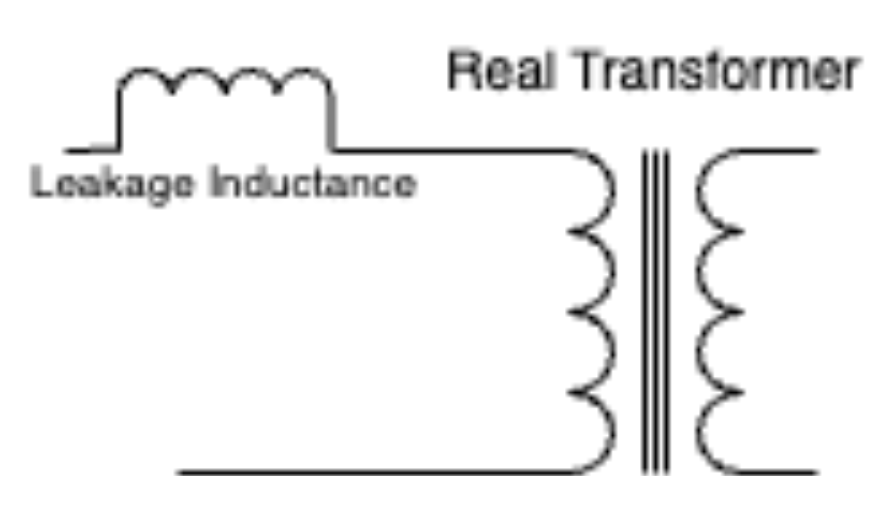
\includegraphics[width=0.3\textwidth]{basic2.png}
    \label{fig:basic2}
\end{figure}

\noindent
So essentially, we require at least one inductor in series and one in parallel with the transformer for the resonant circuit that we will be designing. (We are using these inductors as part of the resonant circuit to reduce the overall cost of the circuit by minimizing the components used)
\begin{figure}[ht]
    \centering
    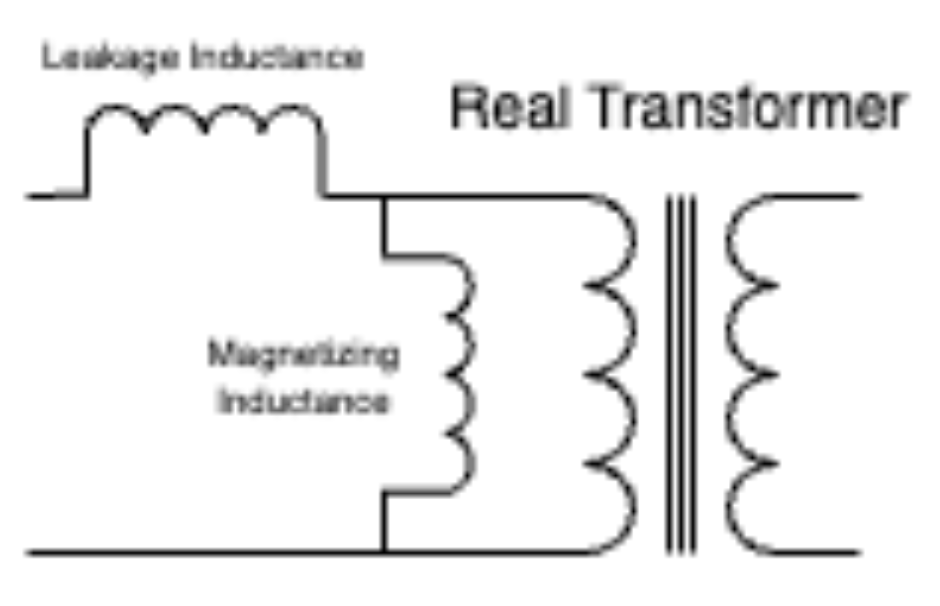
\includegraphics[width=0.3\textwidth]{basic3.png}
    \label{fig:basic3}
\end{figure}

\noindent
Hence, only one configuration of a resonant circuit is possible with two inductors, i.e. an LLC configuration (2 inductors + 1 capacitor)
\begin{figure}[ht]
    \centering
    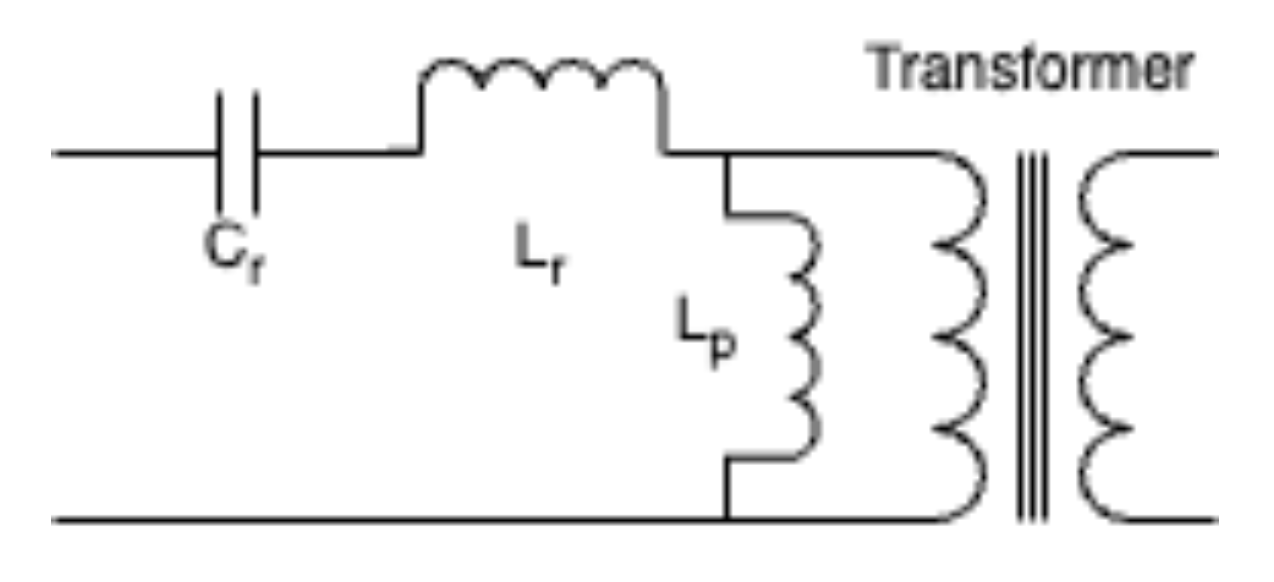
\includegraphics[width=0.3\textwidth]{basic4.png}
    \label{fig:basic4}
\end{figure}

\noindent
Using an LLC Resonant circuit gives us another advantage as well, i.e. the resonant tank circuit (circuit made by the capacitor and the 2 inductors) allows for filtering of the square wave harmonics generated by the switching circuit into a sinewave of fundamental frequency for the transformer.
However, the gain of an LLC Resonant Circuit is dependent on the switching frequency and the load applied across the circuit, hence it needs to be tuned considering the switching frequency and the output load to ensure that the converter efficiently operates across a wide range of loads by designing it such that the tank’s gain is as per our requirements.